\documentclass[landscape]{article}
\usepackage[a4paper,landscape,margin=1.5cm]{geometry}
\usepackage{graphicx}
\usepackage{array}
\usepackage{tabularx}
\usepackage{colortbl}
\usepackage{xcolor}
\usepackage{fancyhdr}
\usepackage{tikz}
\usepackage{booktabs}
\usepackage{subcaption}
\usepackage{pagecolor}
\usepackage{multirow}
\usepackage{lastpage}
\usepackage{tgheros} % Modern sans-serif font
\usepackage{setspace}
\usepackage[T1]{fontenc}
\usepackage{makecell}
\usepackage{enumitem} % Better list control
\usepackage{fontawesome5} % For icons
\usepackage{pdflscape} % Better landscape handling

\graphicspath{{illustration/}{reference/}{figures/}}  % Paths for images

% Define refined color palette
\definecolor{primaryblue}{RGB}{41, 65, 94}   % Deeper blue for main headers
\definecolor{secondaryblue}{RGB}{78, 112, 155} % Lighter blue for secondary elements
\definecolor{lightblue}{RGB}{235, 242, 250} % Very light blue for table backgrounds
\definecolor{mediumblue}{RGB}{120, 150, 180} % Medium blue for table headers
\definecolor{accentgold}{RGB}{216, 181, 109} % Gold accent color
\definecolor{backgroundbeige}{RGB}{252, 250, 245} % Light beige background
\definecolor{tablehead}{RGB}{245, 245, 245} % Subtle gray for table headers
\definecolor{bordercolor}{RGB}{220, 220, 220} % Subtle border color
\definecolor{subtleshadow}{RGB}{240, 240, 240} % For subtle shadows

% Set background color
\pagecolor{white}

% Set document font to sans-serif
\renewcommand{\familydefault}{\sfdefault}

% Better spacing
\setstretch{1.2}
\setlength{\parindent}{0pt}
\setlength{\parskip}{8pt}
\renewcommand{\arraystretch}{1.5} % Improve table row height globally

% Fix for table line alignment
\setlength{\arrayrulewidth}{0.5pt}
\setlength{\tabcolsep}{6pt}

% Custom page style
\pagestyle{fancy}
\fancyhf{}
\renewcommand{\headrulewidth}{0pt}
\renewcommand{\footrulewidth}{0pt}

% Enhanced Header with brand bar and subtle shadow
\fancyhead[C]{%
\begin{tikzpicture}[remember picture, overlay]
    % Shadow effect
    \fill[subtleshadow] 
        ([yshift=-1.2cm, xshift=0.2cm]current page.north west) rectangle 
        ([yshift=-0.8cm, xshift=0.2cm]current page.north east);
    
    % Header bar with gradient
    \shade[top color=primaryblue, bottom color=secondaryblue] 
        ([yshift=-1cm]current page.north west) rectangle 
        ([yshift=0cm]current page.north east);
    
    % Gold accent line
    \fill[accentgold] 
        ([yshift=-1cm]current page.north west) rectangle 
        ([yshift=-0.9cm]current page.north east);
    
    % Brand name with logo placeholder
    \node[anchor=west, text=white, font=\Large\bfseries] 
        at ([xshift=1cm, yshift=-0.5cm]current page.north west) 
        {FASHION BRAND};
    
    % Document type indicator
    \node[anchor=east, text=white, font=\large] 
        at ([xshift=-1cm, yshift=-0.5cm]current page.north east) 
        {TECHNICAL SPECIFICATION};
\end{tikzpicture}%
}

% Enhanced footer with contact info and modern design
\fancyfoot[C]{%
\begin{tikzpicture}[remember picture, overlay]
    % Shadow effect
    \fill[subtleshadow] 
        ([yshift=0.9cm, xshift=0.2cm]current page.south west) rectangle 
        ([yshift=0.2cm, xshift=0.2cm]current page.south east);
    
    % Blue footer bar with gradient
    \shade[bottom color=primaryblue, top color=secondaryblue] 
        ([yshift=0.7cm]current page.south west) rectangle 
        ([yshift=0cm]current page.south east);
    
    % Gold accent line
    \fill[accentgold] 
        ([yshift=0.7cm]current page.south west) rectangle 
        ([yshift=0.65cm]current page.south east);
    
    % Copyright text with icon
    \node[anchor=west, text=white, font=\small] 
        at ([xshift=1cm, yshift=0.35cm]current page.south west) 
        {\faIcon{copyright} FASHION BRAND 2025};
    
    % Contact info in footer
    \node[anchor=center, text=white, font=\small] 
        at ([yshift=0.35cm]current page.south) 
        { \quad };
    
    % Page number with icon
    \node[anchor=east, text=white, font=\small] 
        at ([xshift=-1cm, yshift=0.35cm]current page.south east) 
        {\faIcon{file-alt} PAGE \thepage\ OF \pageref{LastPage}};
\end{tikzpicture}%
}

% Improved section command with shadow effect
\newcommand{\techsection}[1]{%
\noindent\begin{tabularx}{\textwidth}{|X|}
\hline
\cellcolor{primaryblue}\textcolor{white}{\large\textbf{\faIcon{angle-right} #1}} \\
\hline
\end{tabularx}
\vspace{0.1cm}
}

% Command for elevated panels with shadow
\newcommand{\elevatedbox}[1]{%
\begin{tikzpicture}
\node[draw=bordercolor, line width=0.5pt, inner sep=10pt, fill=white, rounded corners=3pt, 
      drop shadow={shadow xshift=1pt, shadow yshift=-1pt, opacity=0.2}] {#1};
\end{tikzpicture}
}

\begin{document}

% Title with enhanced decorative elements and subtle shadow
\begin{center}

\begin{tikzpicture}
% Shadow layer
\node[inner sep=12pt, opacity=0.1, yshift=-2pt, xshift=2pt] (shadow) {\Huge\textbf{\textcolor{black}{Technical Specification Sheet}}};
% Main title
\node[inner sep=12pt] (title) {\Huge\textbf{\textcolor{primaryblue}{Technical Specification Sheet}}};
% Dual accent lines
\draw[accentgold, line width=2pt] ([yshift=-5pt]title.south west) -- ([yshift=-5pt]title.south east);
\draw[secondaryblue, line width=1pt] ([yshift=-9pt]title.south west) -- ([yshift=-9pt]title.south east);
% Icon decorations on both sides
\node[anchor=east, xshift=-10pt] at (title.west) {\textcolor{accentgold}{\Large\faIcon{ruler}}};
\node[anchor=west, xshift=10pt] at (title.east) {\textcolor{accentgold}{\Large\faIcon{cut}}};
\end{tikzpicture}
\end{center}

\vspace{0.5cm}

% PRODUCT DETAILS - Enhanced with icons and better layout
\begin{center}
\begin{tabular}{|>{\bfseries\raggedright\arraybackslash}p{3.2cm}|p{4cm}|>{\bfseries\raggedright\arraybackslash}p{3.2cm}|p{4cm}|}
\hline
\cellcolor{tablehead}\faIcon{tag} Brand: & PLACEHOLDER & \cellcolor{tablehead}\faIcon{user} Designer: & PLACEHOLDER \\
\hline
\faIcon{tshirt} Style Name: & PLACEHOLDER  & \faIcon{hashtag} Style Number: & PLACEHOLDER  \\
\hline
\cellcolor{tablehead}\faIcon{layer-group} Category: & PLACEHOLDER & \cellcolor{tablehead}\faIcon{calendar-alt} Season: & PLACEHOLDER \\
\hline
\faIcon{calendar-day} Date: & PLACEHOLDER  & \faIcon{code-branch} Version: & PLACEHOLDER \\
\hline
\end{tabular}
\end{center}

\vspace{0.5cm}

% PRODUCT DESCRIPTION with elevated design
\begin{center}
\begin{tabular}{|p{14cm}|}
\hline
\rowcolor{tablehead}\multicolumn{1}{|c|}{\textbf{\faIcon{info-circle} PRODUCT DESCRIPTION}} \\
\hline
\vspace{0.2cm}
\large % INSERT PRODUCT DESCRIPTION HERE
\vspace{0.3cm} \\
\hline
\end{tabular}
\end{center}

\newpage

%%START_DRAWING_SECTION%%
% --------------------------------- FRONT VIEW SECTION ---------------------------------
\techsection{FRONT VIEW}
\vspace{-0.3cm}

\begin{tabular}{p{0.49\textwidth}|p{0.49\textwidth}}
% Left side - FRONT VIEW with better frame
\begin{center}
\begin{tikzpicture}
\node[draw=bordercolor, line width=0.5pt, inner sep=4pt, fill=white, rounded corners=3pt] {
    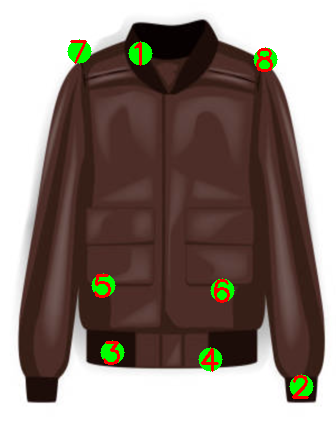
\includegraphics[width=0.35\textwidth,height=12cm,keepaspectratio]{/Users/johncao/Documents/Programming/Stanford/CS224G_V2/CS224G_TechPackAI/demo_images/jacket/jacket_front.png}
};
% Add a small label on top
\node[anchor=north, fill=accentgold, text=white, font=\small\bfseries, rounded corners=2pt, inner sep=2pt] 
    at ([yshift=0.5cm]current bounding box.north) {FRONT VIEW};
\end{tikzpicture}
\end{center}
&
% Right side - Attributes Table FRONT VIEW with improved formatting
\begin{center}
\begin{tabular}{|>{\columncolor{lightblue}\bfseries}p{3.5cm}|p{8cm}|}
\hline
\rowcolor{mediumblue}\multicolumn{1}{|c|}{\textcolor{white}{\textbf{\faIcon{list} Component}}} & \multicolumn{1}{c|}{\textcolor{white}{\textbf{\faIcon{info} Specifications}}} \\
\hline
PLACEHOLDER & PLACEHOLDER \\
PLACEHOLDER & PLACEHOLDER \\
\hline
\end{tabular}
\end{center}
\end{tabular}

\vspace{0.5cm}

% MEASUREMENTS TABLE FRONT VIEW - WITH IMPROVED STYLING
\noindent\begin{tabularx}{\textwidth}{|>{\columncolor{lightblue}\bfseries}X|X|>{\centering\arraybackslash}X|>{\centering\arraybackslash}X|>{\centering\arraybackslash}X|>{\centering\arraybackslash}X|}
\hline
\rowcolor{primaryblue}\multicolumn{6}{|c|}{\textcolor{white}{\large\textbf{\faIcon{ruler-combined} FRONT MEASUREMENTS}}} \\
\hline
\rowcolor{mediumblue}\textcolor{white}{\textbf{Component}} & \textcolor{white}{\textbf{XS}} & \textcolor{white}{\textbf{S}} & \textcolor{white}{\textbf{M}} & \textcolor{white}{\textbf{L}} & \textcolor{white}{\textbf{XL}} \\
\hline
PLACEHOLDER & PLACEHOLDER & PLACEHOLDER & PLACEHOLDER & PLACEHOLDER & PLACEHOLDER \\
\hline
PLACEHOLDER & PLACEHOLDER & PLACEHOLDER & PLACEHOLDER & PLACEHOLDER & PLACEHOLDER \\
\hline
PLACEHOLDER & PLACEHOLDER & PLACEHOLDER & PLACEHOLDER & PLACEHOLDER & PLACEHOLDER \\
\hline
\end{tabularx}
% ---------------------------------------------------------------------------------------------
\newpage

% --------------------------------- BACK VIEW SECTION ---------------------------------
\techsection{BACK VIEW}
\vspace{-0.3cm}

\begin{tabular}{p{0.49\textwidth}|p{0.49\textwidth}}
% Left side - BACK VIEW with better frame
\begin{center}
\begin{tikzpicture}
\node[draw=bordercolor, line width=0.5pt, inner sep=4pt, fill=white, rounded corners=3pt] {
    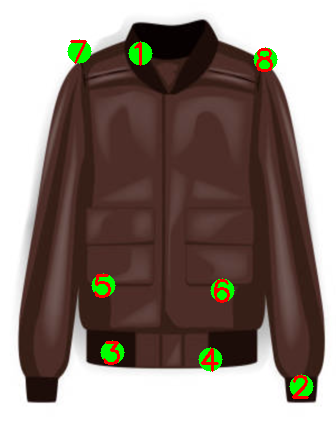
\includegraphics[width=0.35\textwidth,height=12cm,keepaspectratio]{/Users/johncao/Documents/Programming/Stanford/CS224G_V2/CS224G_TechPackAI/demo_images/jacket/jacket_front.png}
};
% Add a small label on top
\node[anchor=north, fill=accentgold, text=white, font=\small\bfseries, rounded corners=2pt, inner sep=2pt] 
    at ([yshift=0.5cm]current bounding box.north) {BACK VIEW};
\end{tikzpicture}
\end{center}
&
% Right side - Attributes Table BACK VIEW with improved formatting
\begin{center}
\begin{tabular}{|>{\columncolor{lightblue}\bfseries}p{3.5cm}|p{8cm}|}
\hline
\rowcolor{mediumblue}\multicolumn{1}{|c|}{\textcolor{white}{\textbf{\faIcon{list} Component}}} & \multicolumn{1}{c|}{\textcolor{white}{\textbf{\faIcon{info} Specifications}}} \\
\hline
PLACEHOLDER & PLACEHOLDER \\
PLACEHOLDER & PLACEHOLDER \\
\hline
\end{tabular}
\end{center}
\end{tabular}

\vspace{0.5cm}

% MEASUREMENTS TABLE BACK VIEW - WITH IMPROVED STYLING
\noindent\begin{tabularx}{\textwidth}{|>{\columncolor{lightblue}\bfseries}X|X|>{\centering\arraybackslash}X|>{\centering\arraybackslash}X|>{\centering\arraybackslash}X|>{\centering\arraybackslash}X|}
\hline
\rowcolor{primaryblue}\multicolumn{6}{|c|}{\textcolor{white}{\large\textbf{\faIcon{ruler-combined} BACK MEASUREMENTS}}} \\
\hline
\rowcolor{mediumblue}\textcolor{white}{\textbf{Component}} & \textcolor{white}{\textbf{XS}} & \textcolor{white}{\textbf{S}} & \textcolor{white}{\textbf{M}} & \textcolor{white}{\textbf{L}} & \textcolor{white}{\textbf{XL}} \\
\hline
PLACEHOLDER & PLACEHOLDER & PLACEHOLDER & PLACEHOLDER & PLACEHOLDER & PLACEHOLDER \\
\hline
PLACEHOLDER & PLACEHOLDER & PLACEHOLDER & PLACEHOLDER & PLACEHOLDER & PLACEHOLDER \\
\hline
PLACEHOLDER & PLACEHOLDER & PLACEHOLDER & PLACEHOLDER & PLACEHOLDER & PLACEHOLDER \\
\hline
\end{tabularx}
% ---------------------------------------------------------------------------------------------
%%END_DRAWING_SECTION%%

\newpage

% REFERENCE IMAGES SECTION with callouts
\techsection{REFERENCE}
\vspace{-0.3cm}

\begin{tabular}{p{0.49\textwidth}|p{0.49\textwidth}}
% Left side - Place reference images with annotations
\begin{center}
\begin{tikzpicture}
\node[draw=bordercolor, line width=0.5pt, inner sep=4pt, fill=white, rounded corners=3pt] (img) {
    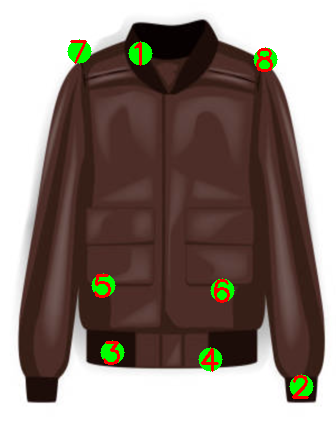
\includegraphics[width=0.35\textwidth,height=12cm,keepaspectratio]{/Users/johncao/Documents/Programming/Stanford/CS224G_V2/CS224G_TechPackAI/demo_images/jacket/jacket_front.png}
};

% Sample callout annotations (uncomment and modify when image is added)
%\draw[accentgold, ->, line width=1pt] (1,1) -- (0.5,0.5) node[right, text=black, font=\small, align=left, xshift=5pt] {Special detail};
%\draw[accentgold, ->, line width=1pt] (-1,1) -- (-0.5,0.5) node[left, text=black, font=\small, align=right, xshift=-5pt] {Stitch detail};

% Add a small label on top
\node[anchor=north, fill=accentgold, text=white, font=\small\bfseries, rounded corners=2pt, inner sep=2pt] 
    at ([yshift=0.5cm]current bounding box.north) {INSPIRATION \& DETAILS};
\end{tikzpicture}
\end{center}
&
% Right side - Description of reference image with enhanced formatting
\begin{center}
\begin{tabular}{|p{10cm}|}
\hline
\rowcolor{mediumblue}\multicolumn{1}{|c|}{\textcolor{white}{\textbf{\faIcon{lightbulb} Design Inspiration \& Notes}}} \\
\hline
\begin{minipage}[t]{\linewidth}
\vspace{0.3cm}
PLACEHOLDER
\begin{itemize}[leftmargin=*, label={\textcolor{accentgold}{\faIcon{check-circle}}}]
  \item PLACEHOLDER
\end{itemize}
\vspace{0.3cm}
\end{minipage} \\
\hline
\end{tabular}
\end{center}
\end{tabular}

\newpage

% BILL OF MATERIALS with enhanced design
\techsection{BILL OF MATERIALS}
\vspace{-0.3cm}
\noindent\begin{tabularx}{\textwidth}{|>{\columncolor{lightblue}\bfseries}p{3cm}|X|>{\raggedleft\arraybackslash}p{2.5cm}|>{\raggedleft\arraybackslash}p{2.5cm}|}
\hline
\rowcolor{mediumblue}\textcolor{white}{\textbf{Material}} & \textcolor{white}{\textbf{Description}} & \textcolor{white}{\textbf{Unit Cost}} & \textcolor{white}{\textbf{Total Cost}} \\
\hline
PLACEHOLDER & PLACEHOLDER  & PLACEHOLDER  & PLACEHOLDER   \\
\hline
PLACEHOLDER & PLACEHOLDER  & PLACEHOLDER  & PLACEHOLDER   \\
\hline
PLACEHOLDER & PLACEHOLDER  & PLACEHOLDER  & PLACEHOLDER   \\
\hline
PLACEHOLDER & PLACEHOLDER  & PLACEHOLDER  & PLACEHOLDER   \\
\hline
\multicolumn{3}{|r|}{\textbf{Total Material Cost:}} & PLACEHOLDER \\
\hline
\end{tabularx}

\vspace{0.7cm}

\newpage

% CARE INSTRUCTIONS with icons
\techsection{CARE INSTRUCTIONS}
\vspace{-0.3cm}

\noindent\begin{tabularx}{\textwidth}{|X|}
\hline
\begin{minipage}[t]{\linewidth}
\vspace{0.3cm}
\large % ENTER CARE INSTRUCTIONS HERE
\begin{center}
\begin{tabular}{ccccc}
\textcolor{primaryblue}{\Large\faIcon{tshirt}} & 
\textcolor{primaryblue}{\Large\faIcon{ban}} & 
\textcolor{primaryblue}{\Large\faIcon{sync}} & 
\textcolor{primaryblue}{\Large\faIcon{temperature-high}} & 
\textcolor{primaryblue}{\Large\faIcon{ban}} \\
Machine Wash & No Bleach & Tumble Dry & Iron Medium & No Dry Clean \\
\end{tabular}
\end{center}

\vspace{0.3cm}
\end{minipage} \\
\hline
\end{tabularx}

\vspace{0.7cm}

% ADDITIONAL COMMENTS with improved formatting
\techsection{ADDITIONAL COMMENTS}
\vspace{-0.3cm}
\noindent\begin{tabularx}{\textwidth}{|X|}
\hline
\begin{minipage}[t]{\linewidth}
\vspace{0.3cm}
\large % ADDITIONAL COMMENT HERE
\end{minipage} \\
\hline
\end{tabularx}

\vspace{0.7cm}
% SIGNATURES
\techsection{SIGNATURES}
\vspace{-0.3cm}
\noindent\begin{tabularx}{\textwidth}{|X|}
\hline
\begin{minipage}[t]{\linewidth}
\vspace{0.3cm}
\large\textbf{Approvals:} \underline{\hspace{5cm}} (Design Director) \hspace{1cm} \underline{\hspace{5cm}} (Production Manager)
\vspace{0.3cm}
\end{minipage} \\
\hline
\end{tabularx}

\newpage

% DISCLAIMER AND CONFIDENTIALITY
\begin{center}
\begin{tabular}{|p{23cm}|}
\hline
\rowcolor{primaryblue}\multicolumn{1}{|c|}{\textcolor{white}{\textbf{DISCLAIMER AND CONFIDENTIALITY}}} \\
\hline
\large % INSERT DISCLAIMER AND CONFIDENTIALITY HERE
\\
\hline
\end{tabular}
\end{center}

\end{document}